\documentclass[14pt, a2paper, landscape, margin=1cm, innermargin=1cm, blockverticalspace=5mm, colspace=5mm, subcolspace=-7mm]{tikzposter}
\tikzposterlatexaffectionproofoff % remove LaTeX TikZposter watermark

% \usetheme{Board}

\title{Posters in \LaTeX\ with \texttt{tikzposter}}

\author{\textbf{Václav Blažej}}
\institute{Faculty of Information Technology, Czech Technical University in Prague, Prague, Czech Republic}
%\titlegraphic{\includegraphics[width=0.1\linewidth]{logo_cvut_en.pdf}}

\usepackage{listings}
\lstdefinestyle{mystyle}{
    language={[LaTeX]TeX},
    basicstyle=\ttfamily
}
\lstset{style=mystyle}

\usepackage{setspace}
\usepackage{amssymb}
\usepackage{blindtext}
\usepackage[backend=biber,style=numeric]{biblatex}
\addbibresource{main.bib}

\graphicspath{{images/}}
\usepackage{enumitem}
\setlist{nosep}
\setlist[itemize]{leftmargin=4mm}

\usepackage{tikz}
\usepackage{tikzpagenodes}
\usetikzlibrary{backgrounds,calc,tikzmark}
\usetikzlibrary{decorations.pathreplacing,shapes.misc}
\pgfdeclarelayer{foreground}
\pgfsetlayers{backgroundlayer,main,foreground}
\tikzset{remember picture} % reference nodes in other pictures
\tikzset{
    show curve controls/.style={
        decoration={
            show path construction,
            curveto code={
                \draw [blue, dashed]
                    (\tikzinputsegmentfirst) -- (\tikzinputsegmentsupporta)
                    node [at end, cross out, draw, solid, red, inner sep=2pt]{};
                \draw [blue, dashed]
                    (\tikzinputsegmentsupportb) -- (\tikzinputsegmentlast)
                    node [at start, cross out, draw, solid, red, inner sep=2pt]{};
            }
        }, decorate
    }
}

%% Math
\newcommand{\N}{\ensuremath{\mathbb{N}}}
\newcommand{\Z}{\ensuremath{\mathbb{Z}}}
\newcommand{\Oh}{\mathcal{O}}


%% Problems
\newcommand{\TSP}{\textsc{Traveling Salesperson Problem}\xspace}
\newcommand{\TSPshort}{\textsc{TSP}\xspace}
\newcommand{\sTSP}{\textsc{Subset \TSPshort}\xspace}
\newcommand{\sTSPshort}{{\sc sub\TSPshort}\xspace}
\newcommand{\WRP}{\textsc{Waypoint Routing Problem}\xspace}
\newcommand{\WRPshort}{\textsc{WRP}\xspace}


%% Parameters
\newcommand{\fes}{\ensuremath{\operatorname{fes}}\xspace}
\newcommand{\vc}{\ensuremath{\operatorname{vc}}\xspace}
\newcommand{\mcp}{\ensuremath{\operatorname{mcp}}\xspace}
\newcommand{\mct}{\ensuremath{\operatorname{mct}}\xspace}
\newcommand{\mcc}{\ensuremath{\operatorname{mcc}}\xspace}
\newcommand{\mdc}{\ensuremath{\operatorname{mdc}}\xspace}
\newcommand{\mlinf}{\ensuremath{\operatorname{mlinf}}\xspace}
\newcommand{\fvs}{\ensuremath{\operatorname{fvs}}\xspace}
\newcommand{\fn}{\ensuremath{\operatorname{fn}}\xspace}
\newcommand{\td}{\ensuremath{\operatorname{td}}\xspace}
\newcommand{\tw}{\ensuremath{\operatorname{tw}}\xspace}
\newcommand{\modulator}{\ensuremath{\operatorname{modul}}\xspace}

%% Running time
\renewcommand{\O}{\ensuremath{\mathcal{O}}}
\newcommand{\poly}{\ensuremath{\operatorname{poly}}}


%% Complexity classes
\renewcommand{\P}{\ensuremath{\mathsf{P}}\xspace}
\newcommand{\NP}{\ensuremath{\mathsf{NP}}\xspace}
\newcommand{\NPh}{\NP-hard\xspace}
\newcommand{\NPhness}{\NP-hardness\xspace}
\newcommand{\NPc}{\NP-complete\xspace}
\newcommand{\NPcness}{\NP-completeness\xspace}
\newcommand{\coNPpoly}{{\rm co}\NP{\rm /poly}\xspace}
\newcommand{\FPT}{\ensuremath{\mathsf{FPT}}\xspace}
\newcommand{\XP}{\ensuremath{\mathsf{XP}}\xspace}
\newcommand{\W}[1][1]{\ensuremath{\mathsf{W[#1]}}\xspace}
\newcommand{\Wh}[1][1]{\W[#1]-hard\xspace}
\newcommand{\Whness}[1][1]{\W[#1]-hardness\xspace}
\newcommand{\WK}[1][1]{\ensuremath{\mathsf{WK[#1]}}\xspace}
\newcommand{\WKh}[1][1]{\WK[#1]-hard\xspace}
\newcommand{\WKc}[1][1]{\WK[#1]-complete\xspace}


%% Custom notation shortcuts
\DeclareMathAlphabet{\mathpzc}{OT1}{pzc}{m}{it}
\newcommand{\budget}{\ensuremath{\mathpzc{b}}} % Budget
\newcommand{\wFn}{\ensuremath{\omega}} % Weight function
\newcommand{\WP}{\ensuremath{W}} % Waypoints set
\newcommand{\cFn}{\ensuremath{\kappa}} % Capacity function

\newcommand{\natBeh}{b^{\operatorname{nat}}}
\newcommand{\emptyBeh}{\ensuremath{(\emptyset,\emptyset)}}
\newcommand{\allBeh}{\ensuremath{\mathcal{B}}}

\newcommand{\Imp}{\ensuremath{\operatorname{imp}}} % Impact
\newcommand{\allImp}{\ensuremath{\mathcal{I}}} % All impacts

%% Misc
\newcommand{\YES}{\emph{yes}\xspace}
\newcommand{\YESi}{\YES-instance\xspace}
\newcommand{\NO}{\emph{no}\xspace}
\newcommand{\NOi}{\NO-instance\xspace}


%%%%%%%%%%%%%%%%%%%%%%%%%%%%%%%%%%%%%%%%%%%%%%%%%%%%%%%%%%%%%%%%%%%%%%%%%%%%%%%%%%%%%%%%%%%%%%%%%%%%
% CUSTOM POSTER STYLE %%%%%%%%%%%%%%%%%%%%%%%%%%%%%%%%%%%%%%%%%%%%%%%%%%%%%%%%%%%%%%%%%%%%%%%%%%%%%%
%%%%%%%%%%%%%%%%%%%%%%%%%%%%%%%%%%%%%%%%%%%%%%%%%%%%%%%%%%%%%%%%%%%%%%%%%%%%%%%%%%%%%%%%%%%%%%%%%%%%
\usecolorstyle[colorOne=white!95!blue,colorTwo=blue!20!black,colorThree=green]{Britain}

\settitle{ \centering \vbox{
% \@titlegraphic \\[\TP@titlegraphictotitledistance] \centering
\color{titlefgcolor} {\bfseries \Huge \sc \@title \par}
\vspace*{1em}
{\large \@author \par}
\vspace*{1em}
{\Large \@institute}
}}

\defineblockstyle{sampleblockstyle}{
    titlewidthscale=1, bodywidthscale=1, titlecenter,
    titleoffsetx=0pt, titleoffsety=0pt, bodyoffsetx=0mm, bodyoffsety=2mm,
    bodyverticalshift=0mm, linewidth=3pt,
    titleinnersep=4mm, bodyinnersep=8mm
}{
    \draw[color=framecolor, fill=blockbodybgcolor, rounded corners=2mm] (blockbody.south west)
    rectangle (blockbody.north east);
    \ifBlockHasTitle
        \draw[color=framecolor, fill=blocktitlebgcolor, rounded corners=2mm, line width=1mm] (blocktitle.south west)
        rectangle (blocktitle.north east);
    \fi
}
\useblockstyle{sampleblockstyle}

\colorlet{myred}{red!50!black}
\colorlet{mygreen}{green!50!black}
\colorlet{myblue}{blue!70!black}

%%%%%%%%%%%%%%%%%%%%%%%%%%%%%%%%%%%%%%%%%%%%%%%%%%%%%%%%%%%%%%%%%%%%%%%%%%%%%%%%%%%%%%%%%%%%%%%%%%%%
%%%%%%%%%%%%%%%%%%%%%%%%%%%%%%%%%%%%%%%%%%%%%%%%%%%%%%%%%%%%%%%%%%%%%%%%%%%%%%%%%%%%%%%%%%%%%%%%%%%%
%%%%%%%%%%%%%%%%%%%%%%%%%%%%%%%%%%%%%%%%%%%%%%%%%%%%%%%%%%%%%%%%%%%%%%%%%%%%%%%%%%%%%%%%%%%%%%%%%%%%

% begin document
\begin{document}
\maketitle[width=.98\textwidth,titletotopverticalspace=5mm,titletoblockverticalspace=5mm,roundedcorners=4mm,linewidth=2mm]
\centering

\begin{columns}
    \column{.25}
    \block{Poster layout}{
        % \begin{lstlisting}
        % \end{lstlisting}
% \\begin\{columns\}
    % \\column\{.25\}
    % \\block\{Poster layout\}\{
    % \}
% \\end\{columns\}
    }
\end{columns}

% \begin{columns}
    % \column{.5}


    % \block{\color{myblue}Traveling Salesperson \subnode{tspdef}{Problem} (\TSPshort)}{
        % \begin{itemize}[leftmargin=26mm]
            % \item[\textbf{Input:}] Simple \textbf{\subnode{weightedtext}{weighted}} undirected graph $G=(V,E,\omega)$, where $\omega\colon E\to\mathbb{N}$ and a \textbf{budget $B\in\mathbb{N}$}.
            % \item[\textbf{Output:}] Is there a \textbf{closed walk} $R$ that visits all vertices and has the total weight at most $B$?
        % \end{itemize}
        % \medskip
        % \begin{itemize}
            % \item \TSPshort is an \NPh problem
            % \item it is \FPT with respect to treewidth
        % \end{itemize}
    % }

    % \column{.5}

    % \block{}{
        % \vspace{-1.23cm}
        % \begin{tikzfigure}
            % \includegraphics[page=2,width=.758\colwidth]{tsp.pdf}
        % \end{tikzfigure}
        % \vspace{-1.1cm}
    % }

% \end{columns}

% \begin{columns}
    % \column{.3}

    % \block{\color{mygreen}Vertex Cover \subnode{vcntext}{Number}}{

        % \begin{itemize}
            % \item vertices outside of the vertex cover $M$ have a cheapest way to connect to $M$
        % \end{itemize}
        % \begin{tikzfigure}
            % 
\includegraphics[page=3,width=.8\colwidth]{behavior.pdf}
        % \end{tikzfigure}
        % \begin{center}
            % {\small connect $u$ with $v$ using a total weight $2$}
        % \end{center}
        % \vspace{-3mm}
        % \begin{itemize}
            % \item connecting all vertices in the cheapest way may not give a connected solution
            % \item ``pay'' an additional fee to some vertices to change their connections so that the solution is connected
        % \end{itemize}
        % \begin{tikzfigure}
            % 
\includegraphics[page=8,width=.8\colwidth]{behavior.pdf}
        % \end{tikzfigure}
        % \begin{center}
            % {\small {\bf\color{orange} pay 1} or {\bf\color{myblue} pay 3} to connect $w$ with $v$}
        % \end{center}
        % \vspace{-3mm}
        % \begin{itemize}
            % \item retain $M$ and a polynomial number of such vertices for each $(v,w)$ pair
            % \item $\to$ {\color{mygreen}polynomial kernel}
        % \end{itemize}
        % % Other vertices are always connected in the cheapest way $\to$
    % }

    % \column{.4}

    % \block{\color{black}Our results}{\rule{0pt}{282mm}}

    % \column{.3}

    % \block{\color{mygreen}F\subnode{fesntext}{}eedback Edge Set No.}{
        % \begin{itemize}
            % \item leaves always have a clear solution
            % \item chains of degree $2$ vertices have the number of possibilities small and can be modelled with smaller subgraphs
            % \item similar reductions also work for the generalized \TSPshort (see box at the bottom)
            % \item exhaustive application gives a {\color{mygreen}polynomial kernel}
        % \end{itemize}
    % }


    % \block{\color{myred}Negative results}{
        % \begin{itemize}
            % \item {\color{myred}{no polynomial kernel}} for \TSPshort with respect to the \textbf{fractioning \subnode{fntext}{number}} unless polynomial hierarchy collapses
            % \item {\color{myred}{no polynomial kernel}} with respect to the combined parameter \textbf{treewidth and maximum de-\subnode{twmaxdegtext}{gree}} unless polynomial hierarchy collapses
            % \item unweighted \sTSP with respect to the \textbf{modulator to dis-\subnode{modcycletext}{joint} cycles} is {\color{myred}\WKh} $\Rightarrow$ {\color{myred}no polynomial kernel}
        % \end{itemize}
    % }

    % \block{}{
        % {
            % % \tiny
            % % \printbibliography[heading=none]
            % \vspace{-17.3mm}
            % \begin{tikzfigure}
                % 
\includegraphics[width=.8\colwidth]{RCI.jpg}
            % \end{tikzfigure}
            % \vspace{-9mm}
            % \tiny
            % \begin{spacing}{1.2}
                % {\tiny The authors acknowledge the support of the OP VVV MEYS funded project CZ.02.1.01/0.0/0.0/16\_019/0000765 ``Research Center for Informatics'' and the Grant Agency of the Czech Technical University in Prague funded grant No.~SGS20/208/OHK3/3T/18.}
            % \end{spacing}
            % \vspace{-3mm}
        % }
    % }

% \end{columns}

% \block{\color{black}Generalizations}{
    % \begin{minipage}[t]{.48\textwidth}
        % % We also consider two generalizations of the problem.
        % \begin{center}
            % \sTSP
        % \end{center}
        % \vspace{-5mm}
        % \begin{itemize}
            % \item has a set of waypoints $W\subseteq V$ (full) that need to be traversed
        % \end{itemize}

        % \begin{minipage}{.65\textwidth}
            % \begin{tikzfigure}
                % \includegraphics[page=7,width=.7\textwidth]{vc_subset.pdf}
            % \end{tikzfigure}
        % \end{minipage}
        % \quad
        % \begin{minipage}{.25\textwidth}
            % \begin{tikzpicture}[scale=.8,main/.style={draw=black,fill=#1!40!white}]
                % \newcommand{\smallboxik}[2]{\draw[main=#1] (#2) rectangle +(1.6,.5);}
                % \newcommand{\smallconnect}[2]{\draw[gray,thick] ($(#1)+(.8,0)$) -- ($(#2)+(.8,.5)$);}
                % \smallboxik{green}{0,3}
                % \smallboxik{green}{0,2}
                % \smallboxik{white}{0,1}
                % \smallboxik{red}{0,0}
                % \smallboxik{green}{2,3}
                % \smallboxik{white}{2,1}
                % \smallboxik{red}{2,0}
                % \smallboxik{red}{1,-1}
                % \node (anotherhardness) at (3.3,0.2){};
                % \smallconnect{0,3}{0,2}
                % \smallconnect{0,2}{0,1}
                % \smallconnect{0,1}{0,0}
                % \smallconnect{2,3}{2,1}
                % \smallconnect{2,1}{2,0}
                % \smallconnect{0,2}{2,1}
                % \smallconnect{0,0}{1,-1}
                % \smallconnect{2,0}{1,-1}
            % \end{tikzpicture}
        % \end{minipage}

        % \begin{itemize}
            % \item enough vertices neighbor $v\not\in W$ $\rightarrow$ reroute the solution through it
            % \item {\color{mygreen}polynomial kernel} w.r.t. the modulator to constant paths
        % \end{itemize}
    % \end{minipage}
    % ~\vrule~~
    % \begin{minipage}[t]{.42\textwidth}
        % \begin{center}
            % \WRP
        % \end{center}
        % \vspace{-5mm}
        % \begin{itemize}
            % \item has a capacity $c\colon E\to \mathbb{N}$ for every edge
        % \end{itemize}
        % \begin{minipage}{.65\textwidth}
            % \begin{tikzfigure}
                % \includegraphics[page=3,width=.7\textwidth]{vc_wrp.pdf}
            % \end{tikzfigure}
        % \end{minipage}
        % \quad
        % \begin{minipage}{.25\textwidth}
            % \begin{tikzpicture}[scale=.8,main/.style={draw=black,fill=#1!40!white}]
                % \newcommand{\smallboxik}[2]{\draw[main=#1] (#2) rectangle +(1.6,.5);}
                % \newcommand{\smallconnect}[2]{\draw[gray,thick] ($(#1)+(.8,0)$) -- ($(#2)+(.8,.5)$);}
                % \smallboxik{green}{0,3}
                % \smallboxik{white}{0,2}
                % \smallboxik{white}{0,1}
                % \smallboxik{red}{0,0}
                % \smallboxik{green}{2,3}
                % \smallboxik{white}{2,1}
                % \smallboxik{red}{2,0}
                % \smallboxik{red}{1,-1}
                % \smallconnect{0,3}{0,2}
                % \smallconnect{0,2}{0,1}
                % \smallconnect{0,1}{0,0}
                % \smallconnect{2,3}{2,1}
                % \smallconnect{2,1}{2,0}
                % \smallconnect{0,2}{2,1}
                % \smallconnect{0,0}{1,-1}
                % \smallconnect{2,0}{1,-1}
            % \end{tikzpicture}
        % \end{minipage}

        % \begin{itemize}
            % \item \WRPshort can be reduced to capacities $1$ (thin) and $2$ (thick)
            % \item {\color{mygreen}polynomial kernel} with respect to the vertex cover number
        % \end{itemize}
    % \end{minipage}

    % \begin{tikzpicture}[overlay, xscale=.85, yscale=1.1, shift={($(current page.center)+(-.2,-2.0)$)}, anchor=center, main/.style={draw=black,fill=#1!40!white,inner sep=4mm}]
        % \newcommand{\cpxboxik}[5]{
            % \node[main={#1},align=center] (#2) at (#3) {\textbf{#4} \\#5};
        % }
        % \cpxboxik{white}{fvsn}{5.5,-1}{Feedback Vertex Set No.}{Remove $k$ vertices so that\\no cycles are left.}
        % \cpxboxik{green}{vc}{-5,9}{Vertex Cover Number}{Remove $k$ vertices to obtain\\an independent set.\\\TSPshort has $\Oh(k^{16})$ kernel.}
        % \cpxboxik{green}{mtcp}{-5,4}{Mod. to Const. Paths}{Remove $k$ vertices to obtain\\contant-length paths\\kernel from $\downarrow$ result}
        % \cpxboxik{green}{mtcc}{-5,-1}{Mod. to Const. Comps.}{\TSPshort has $k^{\Oh(r)}$ kernel\\where $r$ is size of left\\connected components.}
        % \cpxboxik{red}{fn}{-5,-6}{Fractioning Number}{Remove $k$ vertices\\so that components\\ of size $\le k$ remain.\\no polynomial kernel}
        % % \cpxboxik{red}{tw}{0.25,-11}{Treewidth}{}
        % \node at (-6.5,-10.2) { 
\includegraphics[width=1cm]{arxiv.png} };
        % \node at (-6.5,-12){ 
\includegraphics[width=3cm]{qr_arxiv.png} };
        % \node[main={red},align=center] (tw) at (0.25,-11) {\textbf{Treewidth}};
        % \cpxboxik{green}{fesn}{5.5,9}{Feedback Edge Set No.}{Remove $k$ edges so that\\no cycles are left.}
        % \cpxboxik{white}{mtdc}{5.5,-6}{Mod. to Disjoint Cycles}{Remove $k$ vertices so that\\disjoint cycles are left.}
        % \begin{pgfonlayer}{backgroundlayer}
            % \begin{scope}[line width=3mm, gray]
                % \draw (vc.center) -- (mtcp.center) -- (mtcc.center) -- (fn.center) -- (tw.center);
                % \draw (mtcp.center) -- (fvsn.center);
                % \draw (fesn.center) -- (fvsn.center) -- (mtdc.center) -- (tw.center);
            % \end{scope}
            % \begin{scope}[line width=1.2mm,-{stealth'}]
                % \draw[green!50] ($(vc.center)!.4!(vc.west)$) to[out=120,in=-30] ($(vcntext.east)+(0.7,-.8)$);
                % \draw[green!50] ($(fesn.center)!.4!(fesn.east)$) to[out=60,in=210] ($(fesntext.west)+(-1.0,-.5)$);
                % \draw[red!50] plot [smooth,tension=.8] coordinates {($(fn.north east)!.2!(fn.east)$) (3,-3.8) (8.9,-4) ($(fntext.west)+(.1,-.1)$)};
                % \draw[red!50] plot [smooth,tension=.8] coordinates {($(tw.center)!.5!(tw.east)$) (5,-10) (10,-9) (10.9,-6) ($(twmaxdegtext.west)+(.2,+.6)$)};
                % \draw[red!50] plot [smooth,tension=.8] coordinates {($(anotherhardness)+(.2,.2)$) (0,-18) (6,-15) (9,-11) (modcycletext.west)};
            % \end{scope}
        % \end{pgfonlayer}
    % \end{tikzpicture}
% }


\end{document}
